% --
% test bench

\section{Test Bench of best Neural Network Architectures}\label{sec:exp_tb}
\thesisStateNotReady
This section compares the best neural network architectures in terms of noise and shift invariance to fixed self recorded test audio files of the five speech commands with L5 labels.
The length of those audio files is cut, such that by applying a the fixed input frames of \SI{500}{\milli\second}, both end positions consists of at least the half of the audio file information.
This is especially important for the shift invariance.
The noise invariance finds the highest energy region, as described in \rsec{signal_raw} and uses this frame for classification.

% --
% shift invariance

\subsection{Shift invariances}
Shift invariances is very important for speech recognition, for instance the waveform should still be classified to the same class, when shifted a little bit in time.
However the restricted frame size of \SI{500}{\milli\second} makes this task very difficult, as it is already known that not all information might fit into the analytic window, like the \enquote{t} in \enquote{left} or \enquote{right} is often missed.
The figures in this section present a correct classification with a colored pixel and an incorrect with a white pixel.
The examples from the adversarial training section are shown in \rfig{exp_tb_shift_fc3}.
\begin{figure}[!ht]
  \centering
    \subfigure[adv init]{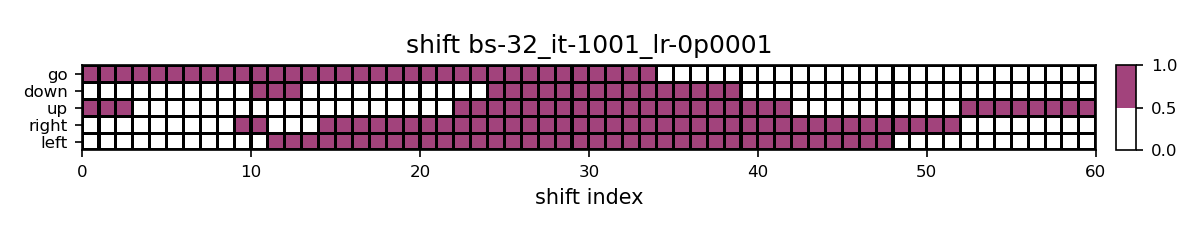
\includegraphics[width=0.45\textwidth]{./5_exp/figs/exp_tb_shift_fc3_adv}}
    \subfigure[random init]{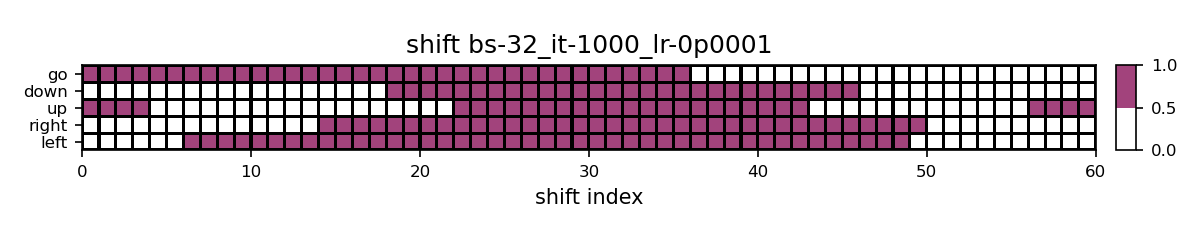
\includegraphics[width=0.45\textwidth]{./5_exp/figs/exp_tb_shift_fc3_random}}
  \caption{Shift invariance of L5-n500, c1d0dd0e0-norm1-it1000-bs32-lr0.0001-mo0.5 once with random init and once with adv init with dec-itl1000.}
  \label{fig:exp_tb_shift_fc3}
\end{figure}
\FloatBarrier
\noindent


% --
% noise invariance

\subsection{Noise invariances}
Noise invariance is a good trait in the classification of speech signals.
That is because the usage of bad microphones or recording set ups may add a lot of noise to the audio and therefore might disturb the classification accuracy.
To create a test upon noise invariance, artificial normal noise is added to the test audio files.
In the plots this is indicated in the x-axis of the plots as Signal to Noise Ration (SNR).
A SNR level of zero means there is equal energy of noise and signal, therefore this signal is already pretty much disturbed.
\rfig{exp_tb_noise_fc3} shows the noise invariance from the example in the adversarial training section.

\begin{figure}[!ht]
  \centering
    \subfigure[adv init]{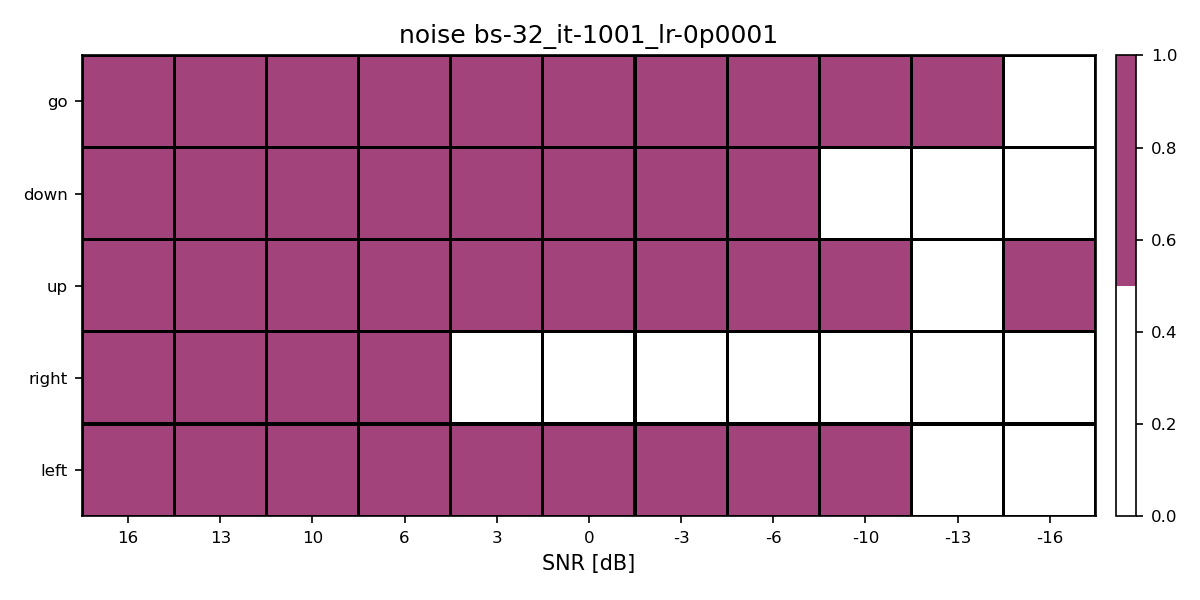
\includegraphics[width=0.40\textwidth]{./5_exp/figs/exp_tb_noise_fc3_adv}}
    \subfigure[random init]{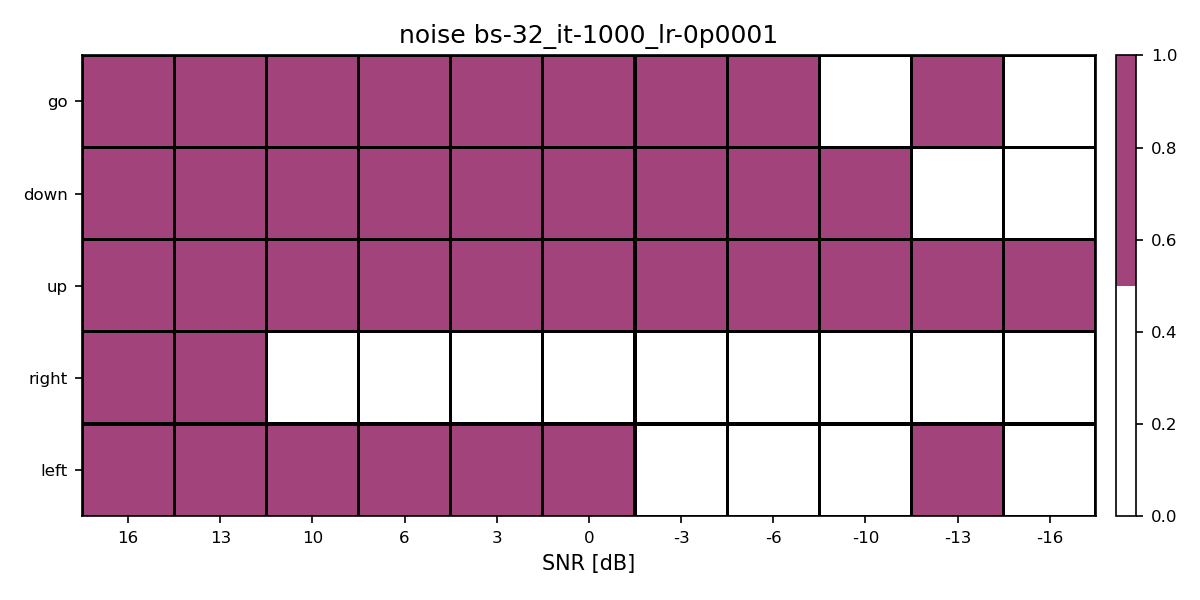
\includegraphics[width=0.40\textwidth]{./5_exp/figs/exp_tb_noise_fc3_random}}
  \caption{Noise invariance of L5-n500, c1d0dd0e0-norm1-it1000-bs32-lr0.0001-mo0.5 once with random init and once with adv init with dec-itl1000.}
  \label{fig:exp_tb_noise_fc3}
\end{figure}
\FloatBarrier
\noindent